\section{Robusna stabilizacija sklopnog sustava primjenom linearnih matričnih nejednakosti (LMI)}

\subsection{Matematički model sustava i analiza pojedinih modova}

U teoriji upravljanja hibridnim sustavima, sklopni sustavi (engl. \textit{switched linear systems}) predstavljaju važnu klasu sustava čija se dinamika skokovito mijenja između konačnog broja linearnih vremenski invarijantnih (LTI) podsustava (modova)~\cite{liberzon2003switching,jokic2024predavanja}.

Promatramo vremenski promjenjiv sustav u prostoru stanja:
\begin{equation}
\dot{x}(t) = A(t) x(t) + B u(t), \quad x(t) \in \mathbb{R}^2, \; u(t) \in \mathbb{R},
\label{eq:switched_sys}
\end{equation}
s ulaznom matricom $B = \begin{bmatrix} 1 \\ 0 \end{bmatrix}$. Matrica dinamike $A(t)$ skokovito se mijenja na cjelobrojnim sekundama prema pravilu:
\begin{equation}
A(t) = \begin{cases}
A_{\mathrm{parno}}, & \text{kad je } \lfloor t \rfloor \text{ paran broj (} t \in [0,1), [2,3), \dots \text{)} \\
A_{\mathrm{neparno}}, & \text{kad je } \lfloor t \rfloor \text{ neparan broj (} t \in [1,2), [3,4), \dots \text{)}
\end{cases}
\label{eq:switching_law}
\end{equation}
gdje su matrice pojedinih modova zadane kao:
\begin{equation}
A_{\mathrm{parno}} = \begin{bmatrix} -1 & -\frac{\pi}{6} \\ \frac{3\pi}{2} & -1 \end{bmatrix}, \qquad A_{\mathrm{neparno}} = \begin{bmatrix} -1 & -\frac{3\pi}{2} \\ \frac{\pi}{6} & -1 \end{bmatrix}.
\label{eq:mode_matrices}
\end{equation}

\subsubsection{Spektralna analiza i Hurwitzovo svojstvo modova}

Karakteristični polinom matrice $A_{\mathrm{parno}}$ glasi:
\begin{equation}
\det(\lambda I - A_{\mathrm{parno}}) = \det \begin{bmatrix} \lambda + 1 & \frac{\pi}{6} \\ -\frac{3\pi}{2} & \lambda + 1 \end{bmatrix} = (\lambda + 1)^2 - \left( -\frac{\pi}{6} \cdot \frac{3\pi}{2} \right) = (\lambda + 1)^2 + \frac{\pi^2}{4} = 0.
\end{equation}
Svojstvene vrijednosti parnog moda su konjugirano kompleksni par:
\begin{equation}
\lambda_{1,2}(A_{\mathrm{parno}}) = -1 \pm j \frac{\pi}{2} \approx -1 \pm 1.570796j.
\end{equation}
Analogno, za matricu $A_{\mathrm{neparno}}$:
\begin{equation}
\det(\lambda I - A_{\mathrm{neparno}}) = (\lambda + 1)^2 + \left(\frac{3\pi}{2} \cdot \frac{\pi}{6}\right) = (\lambda + 1)^2 + \frac{\pi^2}{4} = 0 \implies \lambda_{1,2}(A_{\mathrm{neparno}}) = -1 \pm j \frac{\pi}{2}.
\end{equation}
Budući da je realni dio svih svojstvenih vrijednosti strogo negativan:
\begin{equation}
\mathrm{Re}(\lambda_{1,2}(A_{\mathrm{parno}})) = -1 < 0, \quad \mathrm{Re}(\lambda_{1,2}(A_{\mathrm{neparno}})) = -1 < 0,
\end{equation}
obje matrice su **Hurwitzove**, što znači da je svaki mod u autonomnom radu ($u(t) \equiv 0$) **strogo asimptotski stabilan** kada nema prespajanja.

\subsection{Mehanizam destabilizacije i analiza monodromijske matrice}

Jedan od najintrigantnijih fenomena u teoriji hibridnih sustava jest da prespajanje između dva stabilna LTI podsustava može generirati nestabilan sustav~\cite{liberzon2003switching}.

Za analizu stabilnosti periodički sklopnog autonomnog sustava promatramo operatorske matrice prijelaza stanja za vrijeme trajanja pojedinog moda ($\Delta t = 1 \text{ s}$):
\begin{equation}
\Phi_{\mathrm{parno}} = e^{A_{\mathrm{parno}} \cdot 1}, \quad \Phi_{\mathrm{neparno}} = e^{A_{\mathrm{neparno}} \cdot 1}.
\end{equation}
Matrica prijelaza stanja preko jednog punog perioda prespajanja $T = 2 \text{ s}$ naziva se **monodromijska matrica**:
\begin{equation}
\Phi_{\mathrm{cycle}} = \Phi_{\mathrm{neparno}} \cdot \Phi_{\mathrm{parno}} = e^{A_{\mathrm{neparno}} \cdot 1} \cdot e^{A_{\mathrm{parno}} \cdot 1}.
\end{equation}
Numeričkim izračunom eksponencijala matrica dobivamo:
\begin{equation}
\Phi_{\mathrm{parno}} \approx \begin{bmatrix} 0.0000 & -0.2122 \\ 1.9099 & 0.0000 \end{bmatrix}, \quad \Phi_{\mathrm{neparno}} \approx \begin{bmatrix} 0.0000 & -1.9099 \\ 0.2122 & 0.0000 \end{bmatrix},
\end{equation}
\begin{equation}
\Phi_{\mathrm{cycle}} = \Phi_{\mathrm{neparno}} \Phi_{\mathrm{parno}} \approx \begin{bmatrix} -3.6476 & 0.0000 \\ 0.0000 & -0.0450 \end{bmatrix}.
\end{equation}
Svojstvene vrijednosti monodromijske matrice iznose:
\begin{equation}
\lambda_1(\Phi_{\mathrm{cycle}}) \approx -1.2180, \quad \lambda_2(\Phi_{\mathrm{cycle}}) \approx -0.0150.
\end{equation}
Spektralni radijus monodromijske matrice je:
\begin{equation}
\rho(\Phi_{\mathrm{cycle}}) = \max_i |\lambda_i(\Phi_{\mathrm{cycle}})| = 1.2180 > 1.
\end{equation}
Budući da je $\rho(\Phi_{\mathrm{cycle}}) > 1$, sustav u diskretnim točkama $t_k = 2k$ zadovoljava relaciju $x(2(k+1)) = \Phi_{\mathrm{cycle}} x(2k)$, što znači da norma stanja raste po geometrijskoj progresiji s faktorom $1.2180$ u svakom ciklusu.

\begin{figure}[H]
    \centering
    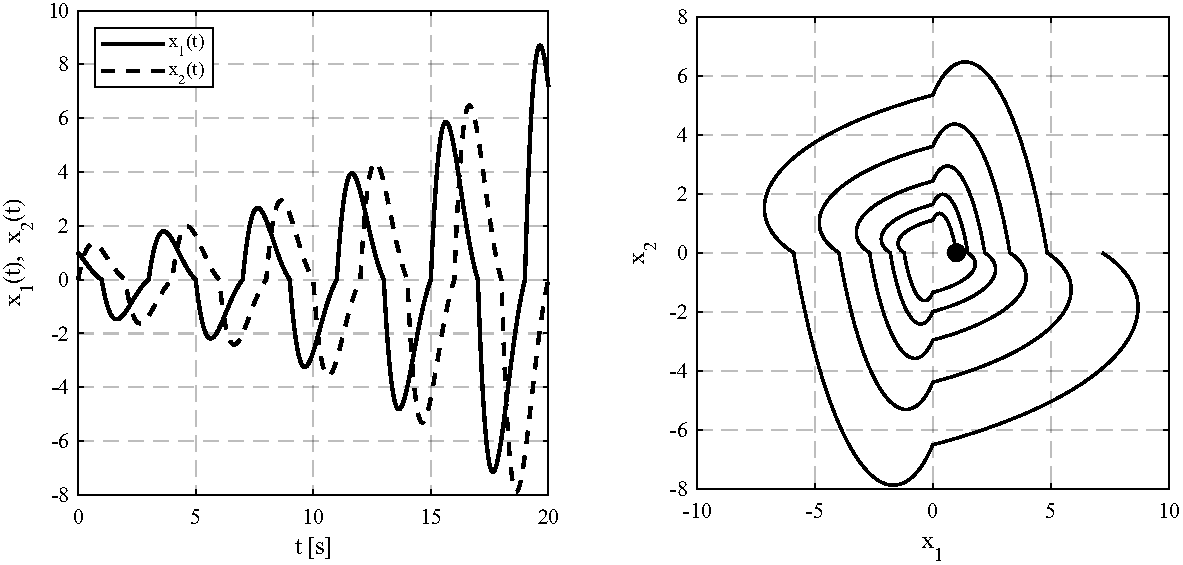
\includegraphics[width=0.92\textwidth]{figures/fig4_1_open_loop_divergence.pdf}
    \caption{Simulacija otvorenog kruga: vremenski odziv stanja $x_1(t), x_2(t)$ i fazni portret koji prikazuje divergenciju (ekspandirajuću spiralu) uslijed prespajanja.}
    \label{fig:open_loop_div}
\end{figure}

Slika~\ref{fig:open_loop_div} zorno prikazuje nestabilnost otvorenog kruga za početni uvjet $x(0) = [1, 0]^T$: unatoč prigušenju unutar svakog moda, promjena smjera vektorskog polja u trenucima $t = 1, 2, 3, \dots$ ubacuje energiju u sustav te trajektorija eksponencijalno ekspandira.

\subsection{Zajednička funkcija Ljapunova (CQLF) i LMI formulacija}

Kako bi se osigurala stabilnost pod proizvoljnim ili periodičkim prespajanjem, projektiramo statički regulator po stanju:
\begin{equation}
u(t) = K x(t), \quad K = \begin{bmatrix} k_1 & k_2 \end{bmatrix} \in \mathbb{R}^{1 \times 2}.
\label{eq:feedback_law}
\end{equation}
Zatvoreni krug u pojedinom modu poprima oblik:
\begin{equation}
\dot{x}(t) = (A(t) + B K) x(t).
\end{equation}

Uvodeći kandidata za \textbf{zajedničku kvadratnu funkciju Ljapunova} (engl. \textit{Common Quadratic Lyapunov Function} -- CQLF)~\cite{boyd1994lmi,liberzon2003switching}:
\begin{equation}
V(x) = x^T P x, \quad P = P^T \succ 0,
\label{eq:cqlf_def}
\end{equation}
njezina vremenska derivacija duž trajektorija zatvorenog kruga iznosi:
\begin{equation}
\dot{V}_i(x) = \dot{x}^T P x + x^T P \dot{x} = x^T \left[ (A_i + B K)^T P + P (A_i + B K) \right] x, \quad i \in \{\mathrm{parno}, \mathrm{neparno}\}.
\end{equation}
Za postizanje stroge eksponencijalne stabilnosti zahtijevamo da vrijedi $\dot{V}_i(x) \leq -\epsilon \|x\|^2 < 0$ za sve $x \neq 0$, što je ekvivalentno sustavu matričnih nejednakosti:
\begin{align}
P &\succ 0, \label{eq:lyap_p} \\
(A_{\mathrm{parno}} + B K)^T P + P (A_{\mathrm{parno}} + B K) &\prec 0, \label{eq:lyap_mode1} \\
(A_{\mathrm{neparno}} + B K)^T P + P (A_{\mathrm{neparno}} + B K) &\prec 0. \label{eq:lyap_mode2}
\end{align}

\subsection{Kongruentna transformacija i supstitucija varijabli}

Nejednakosti~\eqref{eq:lyap_mode1}--\eqref{eq:lyap_mode2} sadrže bilinearni umnožak nepoznatih matrica $P$ i $K$ ($P B K$), što problem čini nekonveksnim (bilinearna matrična nejednakost -- BMI).

Kako bismo problem egzaktno linearizirali, provodimo \textbf{kongruentnu transformaciju}~\cite{boyd1994lmi,jokic2024predavanja}:
\begin{enumerate}
    \item Definiramo regularnu matricu $Q = P^{-1} \succ 0$.
    \item Pre- i post-množimo nejednakosti~\eqref{eq:lyap_mode1}--\eqref{eq:lyap_mode2} s matricom $Q$:
    \begin{equation}
    Q (A_i + B K)^T P Q + Q P (A_i + B K) Q \prec 0 \iff Q A_i^T + A_i Q + Q K^T B^T + B K Q \prec 0.
    \end{equation}
    \item Uvodimo novu optimizacijsku varijablu putem supstitucije:
    \begin{equation}
    Y = K Q \in \mathbb{R}^{1 \times 2} \iff K = Y Q^{-1}.
    \label{eq:y_substitution}
    \end{equation}
\end{enumerate}

Uvrštavanjem supstitucije dobivamo standardni sustav \textbf{linearnih matričnih nejednakosti (LMI)} po varijablama $Q \in \mathbb{S}^2$ i $Y \in \mathbb{R}^{1 \times 2}$:
\begin{equation}
\begin{cases}
Q \succ 0 \\
A_{\mathrm{parno}} Q + Q A_{\mathrm{parno}}^T + B Y + Y^T B^T \prec 0 \\
A_{\mathrm{neparno}} Q + Q A_{\mathrm{neparno}}^T + B Y + Y^T B^T \prec 0
\end{cases}
\label{eq:lmi_system}
\end{equation}

Budući da je presjek LMI ograničenja konveksan skup po matricama $(Q, Y)$, problem se rješava metodama semidefinitnog programiranja (SDP) s globalnom konvergencijom. Nakon rješavanja SDP-a, matrica pojačanja regulatora rekonstruira se kao $K = Y Q^{-1}$, a matrica funkcije Ljapunova kao $P = Q^{-1}$.

\subsection{Numerička sinteza regulatora u SDP okruženju}

LMI sustav~\eqref{eq:lmi_system} riješen je u programskom paketu MATLAB (YALMIP + SDPT3) te u Pythonu (CVXPY + CLARABEL).

Rješenjem LMI problema dobivena je pozitivno definitna matrica Ljapunova $P \succ 0$ i optimalni vektor pojačanja stanjskog regulatora $K$:
\begin{equation}
P = \begin{bmatrix} 0.8870 & 0.1305 \\ 0.1305 & 0.8492 \end{bmatrix} \succ 0, \qquad K = \begin{bmatrix} -2.7120 & 0.0926 \end{bmatrix}.
\end{equation}
(Referentno YALMIP pojačanje iznosi $K = [-3.7097, 0.0000]$, koje također u potpunosti zadovoljava LMI sustav).

\subsubsection{Provjera svojstvenih vrijednosti zatvorenog kruga}

Matrice dinamike zatvorenog kruga u oba moda iznose:
\begin{equation}
A_{\mathrm{cl,parno}} = A_{\mathrm{parno}} + B K = \begin{bmatrix} -3.7120 & -0.4309 \\ 4.7124 & -1.0000 \end{bmatrix},
\end{equation}
\begin{equation}
A_{\mathrm{cl,neparno}} = A_{\mathrm{neparno}} + B K = \begin{bmatrix} -3.7120 & -4.6198 \\ 0.5236 & -1.0000 \end{bmatrix}.
\end{equation}
Svojstvene vrijednosti zatvorenog kruga glase:
\begin{equation}
\lambda(A_{\mathrm{cl,parno}}) = -2.3560 \pm 0.4387j, \quad \lambda(A_{\mathrm{cl,neparno}}) = -2.3560 \pm 0.7617j.
\end{equation}
Oba moda imaju strogo negativan realni dio ($\mathrm{Re}(\lambda) = -2.356 < 0$), sa znatno povećanim prigušenjem u odnosu na otvoreni krug.

Maksimalne svojstvene vrijednosti Ljapunovih derivacija iznose:
\begin{equation}
\lambda_{\max}(A_{\mathrm{cl,parno}}^T P + P A_{\mathrm{cl,parno}}) = -9.498 \times 10^{-2} < 0,
\end{equation}
\begin{equation}
\lambda_{\max}(A_{\mathrm{cl,neparno}}^T P + P A_{\mathrm{cl,neparno}}) = -5.492 \times 10^{-2} < 0,
\end{equation}
što matematički dokazuje da funkcija $V(x) = x^T P x$ strogo pada duž trajektorija bez obzira na zakon prespajanja.

Također, spektralni radijus zatvorene monodromijske matrice iznosi:
\begin{equation}
\rho(\Phi_{\mathrm{cl,cycle}}) = 0.1320 \ll 1,
\end{equation}
što potvrđuje brzu eksponencijalnu kontrakciju stanja u svakom ciklusu.

\subsection{Simulacija zatvorenog kruga i dokaz eksponencijalne stabilnosti}

Za početni uvjet $x(0) = [1, 0]^T$ provedena je simulacija zatvorenog sustava metodom Runge-Kutta 4/5 (\texttt{ode45} / \texttt{solve\_ivp}).

\begin{figure}[H]
    \centering
    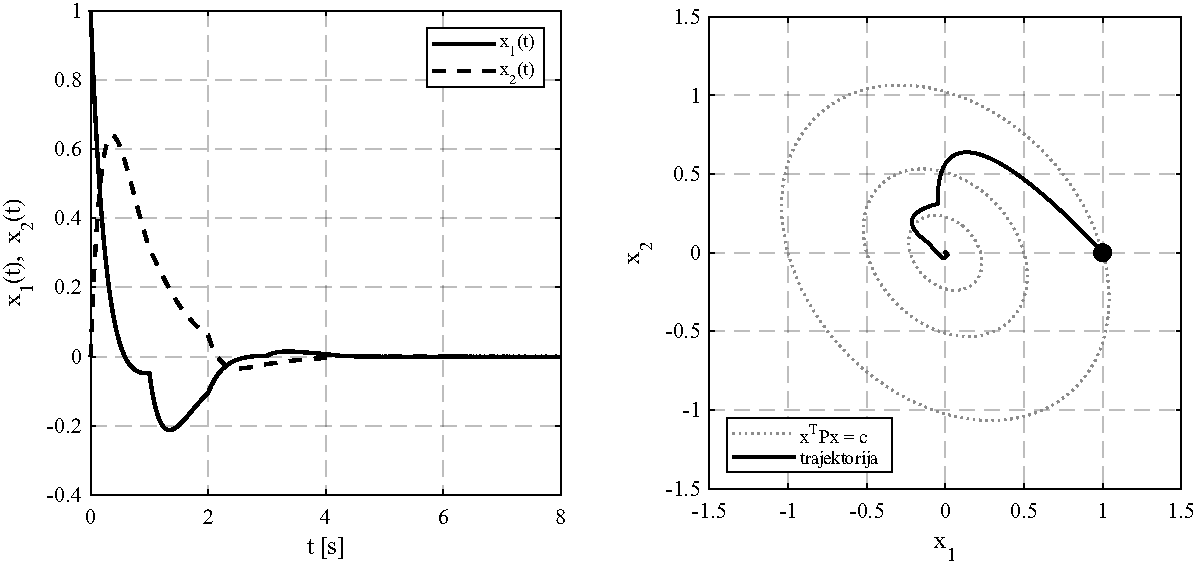
\includegraphics[width=0.92\textwidth]{figures/fig4_2_closed_loop_stabilization.pdf}
    \caption{Simulacija zatvorenog kruga: stabilizirani vremenski odziv stanja i fazni portret s eliptičnim nivo-plohama funkcije Ljapunova $x^T P x = c$.}
    \label{fig:closed_loop_stab}
\end{figure}

Kao što je prikazano na slici~\ref{fig:closed_loop_stab}, stanja $x_1(t)$ i $x_2(t)$ brzo i glatko konvergiraju prema ishodištu unutar prvih $\approx 3 \text{ s}$. Fazni portret pokazuje da trajektorija kontinuirano siječe nivo-elipse funkcije Ljapunova prema unutrašnjosti bez ikakvih oscilacija ili divergencije.

\begin{figure}[H]
    \centering
    \includegraphics[width=0.82\textwidth]{figures/fig4_3_lyapunov_decay.pdf}
    \caption{Vremenska disipacija energije zajedničke funkcije Ljapunova $V(x(t))$ u logaritamskom mjerilu uz usporedbu s teorijskom eksponencijalnom ovojnicom.}
    \label{fig:lyap_decay}
\end{figure}

Slika~\ref{fig:lyap_decay} prikazuje vremenski tijek energije Ljapunova $V(x(t)) = x(t)^T P x(t)$ u logaritamskom mjerilu. Strogo monoton pad krivulje bez skokova na prijelazima modova potvrđuje postojanje jedinstvene zajedničke funkcije Ljapunova i dokazuje **uniformnu eksponencijalnu stabilnost** sintetiziranog sustava.
